\begin{refsection}
\chapter{How Does Multigrid Succeed?}\label{ch:success}

\section{Single-level Solves}

If we run a purely local solver, such as SOR, we see that the error (and residual) initially decrease quickly as we accurately solve local problems.
\begin{bash}
  ./poisson -potential_petscspace_degree 1 -dm_plex_box_faces 16,16 -dm_refine_hierarchy 3 \
    -ksp_type richardson -ksp_rtol 1e-10 -pc_type sor -ksp_type richardson -ksp_max_it 500 \
    -ksp_monitor_error draw::draw_lg -ksp_monitor_pause_final
\end{bash}
However, we need increasingly distant data to make more progress, and the solver is only able to increase its reach by about one adjacent dof per iteration. Thus, we see a rapid slowdown and stagnation of the solve in Fig.~\ref{fig:errorSOR}. Note also that the error has distinct large scale features. These are the low frequency modes that are difficult to eliminate with a purely local solver.

\begin{figure}
\centering
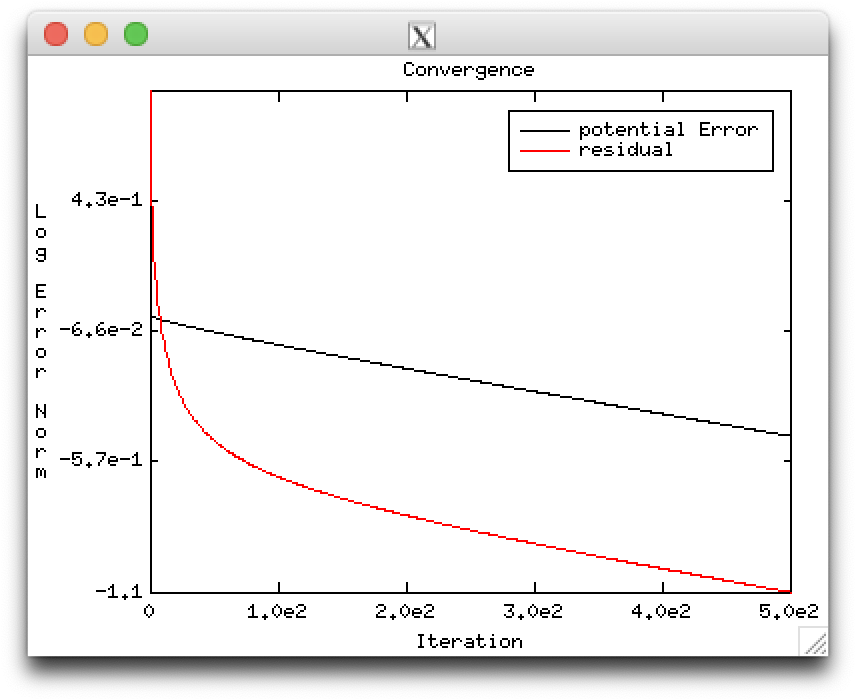
\includegraphics[width=2in]{figures/errorSORLG.png}\hfil
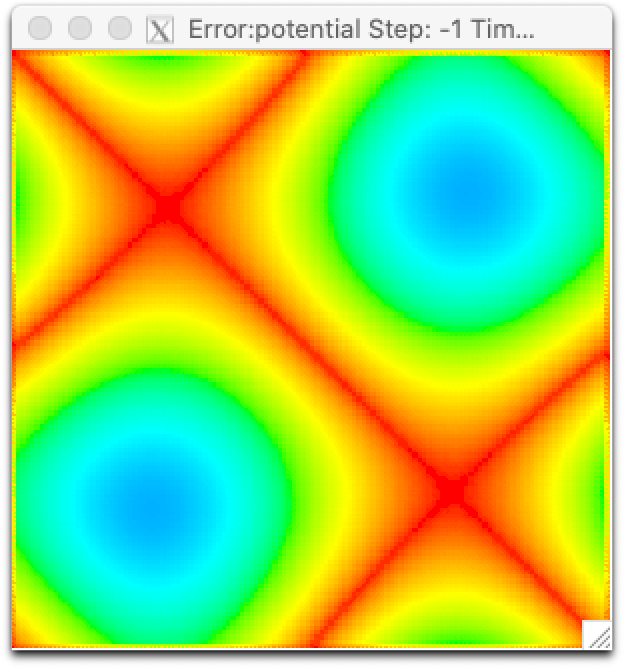
\includegraphics[width=2in]{figures/errorSORLast.png}
\caption{Plot of error norm for each iterate of an SOR solve on the left, and the error itself for the last iterate on the right\label{fig:errorSOR}}
\end{figure}

If we augment SOR with a Krylov solver, we can see that for smaller problems this is enough to converge, as in the left side of Fig.~\ref{fig:errorCGSOR}.
\begin{bash}
  ./poisson -potential_petscspace_degree 1 -dm_plex_box_faces 16,16 -dm_refine_hierarchy 3 \
    -ksp_type cg -ksp_rtol 1e-10 -pc_type sor -ksp_type richardson -ksp_max_it 500 \
    -ksp_monitor_error draw::draw_lg -ksp_monitor_pause_final
\end{bash}
but if we just increase the problem size a little with \bashinline{-dm_refine_hierarchy 6} then the stagnation returns. Asymptotically, Krylov solvers with local preconditioners make no progress at all on this problem.

\begin{figure}
\centering
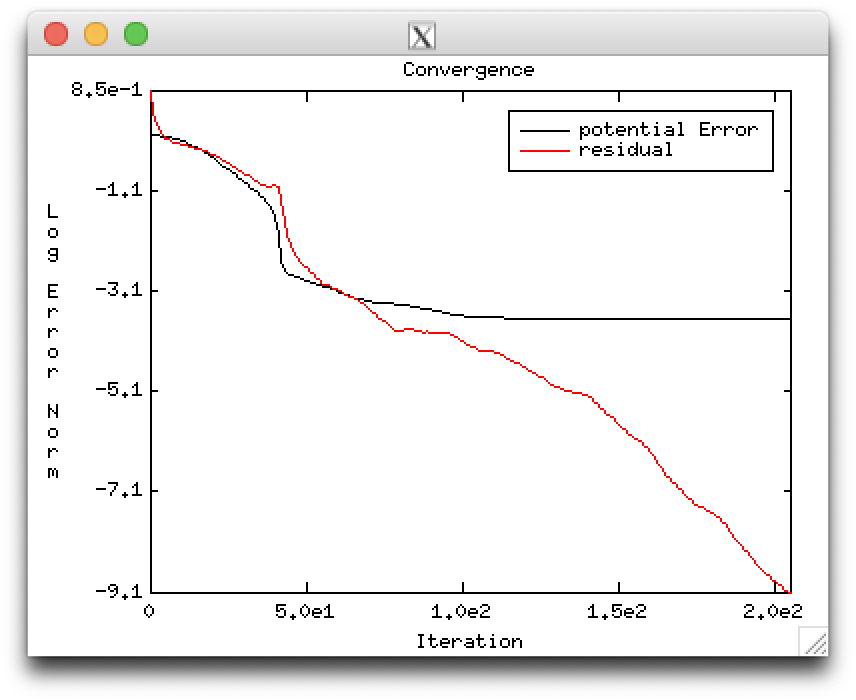
\includegraphics[width=2in]{figures/errorCGSORLG_r3.png}\hfil
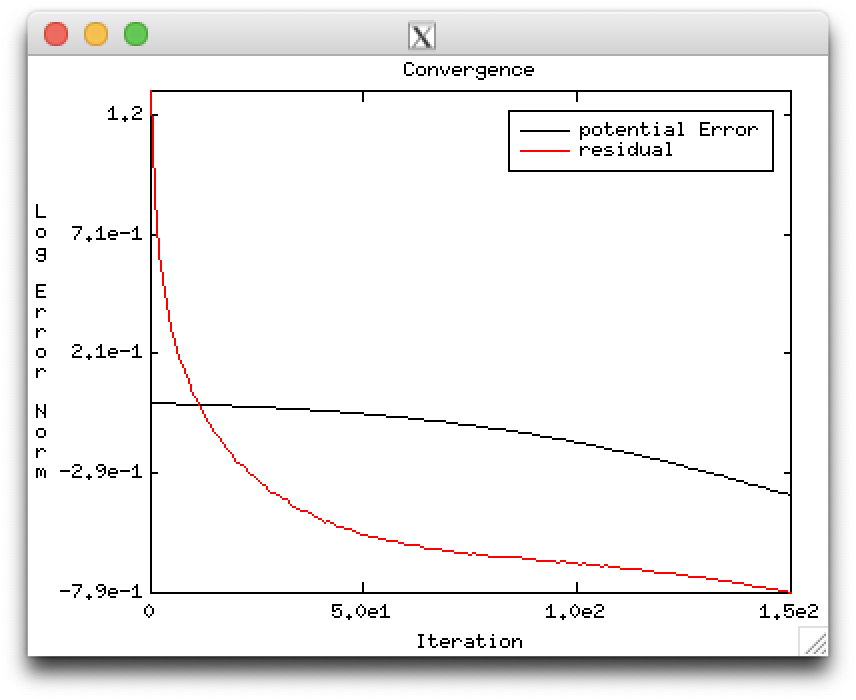
\includegraphics[width=2in]{figures/errorCGSORLG_r6.png}
\caption{Plot of error norm for each iterate of an CG/SOR solve, with 3 refinements on the left and 6 refinements on the right.\label{fig:errorCGSOR}}
\end{figure}

Explain linear convergence and how to calculate the rate.

\section{Multilevel Solves}

Our multigrid will function properly if, at each level, the error component not eliminated by the smoother are eliminated by the coarse solver. Thus, we could start by dividing the space into coarse modes, supported on the coarse mesh, and the remaining fine modes, and then design solvers to handle these two components. However, a design methodology for the solvers is not clear to us. Instead, we will first select a smoother, and then adapt the coarse space to catch error components not handled by the fine solve. The smoother will certainly be local, but can be selected for other properties, such as preservation of a null space~\parencite{FarrellMitchellWechsung2018,FarrellKnepleyWechsungMitchell2020}.

In~\parencite{BrannickEtAl2018}, the authors characterize the optimal coarse grid space, which is the $n$ eigenvectors of lowest eigenvalue for the generalized eigenproblem
\begin{align}
  A \vb{x} = \lambda \tilde M \vb{x}
\end{align}
where $\tilde M$ is the symmetrized smoothing operator, but we will drop the tilde from now on. The idea is that iterative smoothers capture best the modes for large eigenvalues of $M^{-1} A$, and thus we should design our coarse space $\mathcal{P}$ to support the lowest modes of this operator. The space handled well by the smoother is called $\mathcal{S}$, and is the $M$-orthogonal complement of the coarse space $\mathcal{P}$. The important point to keep in mind here is that the optimal coarse space \textit{depends on} the smoother, so it does not make much sense to evaluate them independently.

If the coarse space captures modes not handled by the smoother, prolongation is accurate for these modes, and prolongation also does not dump too much energy in the modes the smoother does handle, then convergence will be rapid. Suppose that I had the exact solution in the coarse space. I would prolong this into the original fine space and then run the smoother. If the error is reduced quickly, without disturbing the coarse solution, then the smoother and coarse space are working well together. In short, if we smooth in the complement of the coarse space, we want to see rapid convergence. This kind of smoothing is called \defineTerm{compatible relaxation}~\parencite{Brandt2000,BrannickFalgout2007} (CR), and one cycle can be written
\begin{align}
  \vb{v}_{k+1} = \left( I - S (S^T M S)^{-1} S^T A \right) \vb{v}_k.
\end{align}
Since $R S = 0$, we can write the whole thing as
\begin{align}
  \vb{v}_{k+1} = \left( I - M_S^{-1} A_S \right) \vb{v}_k.
\end{align}
where $A_S = S^T A S$ and likewise for $M$, as shown in~\parencite{BrannickEtAl2018}. In this \href{https://www.ima.umn.edu/materials/2010-2011/W11.29-12.3.10/10309/ima-2010-cr-v3.pdf}{nice talk} by Rob Falgout, we suggests that the CR iteration should have a convergence rate of about 0.7. Above this, the coarse grid might be missing things.

Here is the monitor output from our Poisson run with constant coefficient, where we calculate the convergence rate $r_V$ for each V-cycle.
\begin{bash}
  0 SNES Function norm 4.525655418801e+01   Rate
    0 KSP Residual norm 9.984017906980e+02
    1 KSP Residual norm 1.180567977130e+01  0.012
    2 KSP Residual norm 2.332568775645e+00  0.20
    3 KSP Residual norm 4.124747107685e-01  0.18
    4 KSP Residual norm 6.605608734491e-02  0.16
    5 KSP Residual norm 1.195672600240e-02  0.18
    6 KSP Residual norm 1.532925985255e-03  0.13
    7 KSP Residual norm 2.442640618761e-04  0.16
    8 KSP Residual norm 4.660857239237e-05  0.19
    9 KSP Residual norm 5.762600750047e-06  0.12
   10 KSP Residual norm 5.834713047805e-07  0.10
   11 KSP Residual norm 1.505628327212e-07  0.26
  1 SNES Function norm 6.902366392273e-09
\end{bash}
so we have a pretty good contraction rate for the V-cycle. We can turn on a CR computation at each level on the homogeneous equation $A x = 0$, and a monitor on the CR iteration to give the convergence rate, using
\begin{bash}
  -pc_mg_adapt_cr
  -mg_levels_cr_ksp_max_it 5 -mg_levels_cr_ksp_converged_rate
    -mg_levels_cr_ksp_converged_rate_type error
\end{bash}
Below, we can see that the CR iterations are converging well on each level for the first few iterations, and it continues in this way until convergence.
\begin{bash}
  0 SNES Function norm 4.525655418801e+01
              Linear mg_levels_1_cr_ solve converged due to CONVERGED_ITS iterations 5 error rate 0.671787 R^2 0.960782
            Linear mg_levels_2_cr_ solve converged due to CONVERGED_ITS iterations 5 error rate 0.642287 R^2 0.976622
          Linear mg_levels_3_cr_ solve converged due to CONVERGED_ITS iterations 5 error rate 0.642214 R^2 0.973073
        Linear mg_levels_4_cr_ solve converged due to CONVERGED_ITS iterations 5 error rate 0.646824 R^2 0.974903
      Linear mg_levels_5_cr_ solve converged due to CONVERGED_ITS iterations 5 error rate 0.645552 R^2 0.975915
    Linear mg_levels_6_cr_ solve converged due to CONVERGED_ITS iterations 5 error rate 0.645276 R^2 0.976259
    0 KSP Residual norm 9.984017906980e+02
              Linear mg_levels_1_cr_ solve converged due to CONVERGED_ITS iterations 5 error rate 0.671787 R^2 0.960782
            Linear mg_levels_2_cr_ solve converged due to CONVERGED_ITS iterations 5 error rate 0.642287 R^2 0.976622
          Linear mg_levels_3_cr_ solve converged due to CONVERGED_ITS iterations 5 error rate 0.642214 R^2 0.973073
        Linear mg_levels_4_cr_ solve converged due to CONVERGED_ITS iterations 5 error rate 0.646824 R^2 0.974903
      Linear mg_levels_5_cr_ solve converged due to CONVERGED_ITS iterations 5 error rate 0.645552 R^2 0.975915
    Linear mg_levels_6_cr_ solve converged due to CONVERGED_ITS iterations 5 error rate 0.645276 R^2 0.976259
    1 KSP Residual norm 1.180567977130e+01
              Linear mg_levels_1_cr_ solve converged due to CONVERGED_ITS iterations 5 error rate 0.671787 R^2 0.960782
            Linear mg_levels_2_cr_ solve converged due to CONVERGED_ITS iterations 5 error rate 0.642287 R^2 0.976622
          Linear mg_levels_3_cr_ solve converged due to CONVERGED_ITS iterations 5 error rate 0.642214 R^2 0.973073
        Linear mg_levels_4_cr_ solve converged due to CONVERGED_ITS iterations 5 error rate 0.646824 R^2 0.974903
      Linear mg_levels_5_cr_ solve converged due to CONVERGED_ITS iterations 5 error rate 0.645552 R^2 0.975915
    Linear mg_levels_6_cr_ solve converged due to CONVERGED_ITS iterations 5 error rate 0.645276 R^2 0.976259
    2 KSP Residual norm 2.332568775645e+00
              Linear mg_levels_1_cr_ solve converged due to CONVERGED_ITS iterations 5 error rate 0.671787 R^2 0.960782
            Linear mg_levels_2_cr_ solve converged due to CONVERGED_ITS iterations 5 error rate 0.642287 R^2 0.976622
          Linear mg_levels_3_cr_ solve converged due to CONVERGED_ITS iterations 5 error rate 0.642214 R^2 0.973073
        Linear mg_levels_4_cr_ solve converged due to CONVERGED_ITS iterations 5 error rate 0.646824 R^2 0.974903
      Linear mg_levels_5_cr_ solve converged due to CONVERGED_ITS iterations 5 error rate 0.645552 R^2 0.975915
    Linear mg_levels_6_cr_ solve converged due to CONVERGED_ITS iterations 5 error rate 0.645276 R^2 0.976259
    3 KSP Residual norm 4.124747107685e-01
\end{bash}

\section{MiniProjects}

Use FFT to calculate the projection onto the eigenbasis for the Laplacian
\begin{itemize}
  \item Project the error to show smoother decreasing coefficients of high frequencies
  \item Project error onto coarse space to show that it captures modes with appreciable coefficients
  \item Project corrected solution to show that mostly high modes are left
\end{itemize}

Use SLEPc to calculate the generalized eigenmodes
\begin{itemize}
  \item Project the error to show smoother decreasing coefficients of high frequencies
  \item Project error onto coarse space to show that it captures modes with appreciable coefficients
  \item Project corrected solution to show that mostly high modes are left
\end{itemize}

Create monitor to display projected error

\printbibliography[heading=subbibliography] % print section bibliography
\end{refsection}
